\documentclass[a4paper,12pt]{article}
\pagestyle{headings}
\usepackage[utf8]{inputenc}
\usepackage{aeguill} 
\usepackage{wrapfig}
\usepackage{graphicx}
\graphicspath{ {project_proposal_img/} }
 


\begin{document}

\begin{titlepage}
\begin{center}

% Upper part of the page. The '~' is needed because \\
% only works if a paragraph has started.
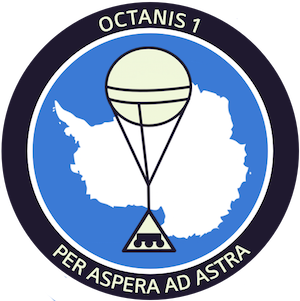
\includegraphics[width=0.35\textwidth]{patch}~\\[2cm]

\textsc{\Large Project Proposal}\\[0.5cm]

% Title
\huge \bfseries Octanis 1: A low-cost autonomous rover for Antarctica permitting real-time sensor data transfer \\[0.4cm] 

% Author and supervisor
\textsc{\small Sam Sulaimanov, Ana Roldàn, Raffael Tschui, Pamela Canjura}
 

\vfill

% Bottom of the page
{\large \today}

\end{center}
\end{titlepage}




\section{Introduction}
»octanis | discovery and exploration« \cite{octanis} is a student initiative to embark on ambitious and challenging projects together as multi-disciplinary students. Octanis 1 is our first mission to build a low-cost autonomous rover for polar, snow or ice covered regions. In this first iteration we will be specialising the rover for the coastal regions of Antarctica and its specific weather conditions. The rover will transmit sensor data like temperature, air pressure, relative humidity, current position and pose. Other more specific enviromental data collection is possible, but needs to be specially addressed due to the non-negligable power and weight requirements. These could be the concentration of an atmospheric gas, $\alpha, \beta, \gamma$ radiation levels or snow and ice sampling. \\ We have selected the periodic sampling of snow and ice to be the best science mission for Octanis 1 \cite{krishnakant}. The rover will have a small hollow device capabale of drilling into the surface ice or snow, melting the sample and analysing the pH.
\\ Octanis 1 will have  Energy will be provided by the solar panels on Octanis' surfaces



\section{Mission Overview}

The aim of this mission, Octanis 1, is to provide a low-cost, low environmental impact rover platform for scientific experiments in cold to extremely cold environments. The rover will be small and light-weight enough to be carried on weather balloons. Its design will allow it to traverse icy terrain and be resistant to wind gusts. It will generate its own power with solar panels and regulate internal temperature as it's first priority. The rover will be on a four-wheel drive platform, each wheel being on a controllable strut, allowing it to drive in any orienation and "stand back up" should it tip over.


\subsection{Objectives}

\paragraph{Robotics}

\paragraph{Deployment}

\paragraph{Sensing}



WP1 Airborne platform:
- Long-range High Altitude Balloon: Reach Antarctica
- Transmit telemetry and experiment data in real time
- Payload is autonomous for an extended period of time (up to 6 months) and can be tracked

WP2 Chemistry:
- Conduct a chemical experiment on-board a high altitude balloon flight to measure the […] of the atmosphere at different altitudes.

WP3 Robotics:
- Rover concept: Balloon is piggybacked to Antarctica by a rover platform. Rover is landed by a parachute if the landing perimeter is allowed to be large. Other landing concepts include a delta glider 




\subsection{Team}

We are a group of students willing to challenge ourselves to the limit. Octanis 1 will not only be built by us, but with many helping professors and advisors that we will meet along the course of the mission. The following presentation is therefore one of the core team:


\paragraph{Sam Sulaimanov} 
\begin{wrapfigure}{l}{0.2\textwidth}
    \centering
    \vspace{-13pt}
    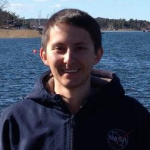
\includegraphics[width=0.15\textwidth]{sam}
\end{wrapfigure} has seven years of experience working as a programmer and communications network engineer. He has been working with microcontrollers and electronics since he was a little boy and will make sure Octanis' brain functions correctly.
\\ \\

\begin{wrapfigure}{l}{0.2\textwidth}
    \centering
    \vspace{-13pt}
    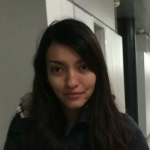
\includegraphics[width=0.15\textwidth]{ana}
\end{wrapfigure}
\paragraph{Ana Roldàn} is a passionate physicist-to-be and involved in every corner of the project. She is not afraid to ask the big questions and inspires everyone with her strong passion for science.
\\ \\

\begin{wrapfigure}{l}{0.2\textwidth}
     \centering
     \vspace{-13pt}
    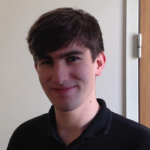
\includegraphics[width=0.15\textwidth]{raf}
\end{wrapfigure} 
\paragraph{Raffael Tschui} is an Electrical Engineer, EPFL, B. Sc. He has the vital role of energy generation, control and regulation in the project. He keeps the rovers heart beating. He is currently on a mission in Columbia to help an EPFL professor build a bio-reactor.
\\ \\

\begin{wrapfigure}{l}{0.2\textwidth}
    \centering
    \vspace{-13pt}
    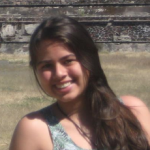
\includegraphics[width=0.15\textwidth]{pam}
\end{wrapfigure} 
\paragraph{Pamela Canjura} has been interested in chemistry since she was five and competes regularly in the Chemistry Olympics. She is working on the chemical analyses that can be done on-board Octanis.
\\ \\


\subsection{Budget}



\section{Rover Transportation and Deployment}

\subsection{Environmental Sustainability}
It is desireable to not leave any waste behind as well as it is required by the Antarctic Treaty. Depending on the method of deployment, the total mass and types of materials that will be included on a mission to Antarctica vary. A deployment of the rover to a target out of reach of normal Antarctic expeditions is done by using a High Altitude Balloon or a standard 3kg latex weather balloon. In such a long-distance mission, the rover will be seperated from the balloon at the target location and the balloon will continue to fly unattended. Therefore the landing location of the balloon can not be known. Due to the nature of such a long-distance mission, typically the rover is unreachable to any expedition or base - the rover is left for the benefit of information on that location.

In a first step, it is therefore proposed to select a landing site that is in reach of normal Antarctic expeditions or bases. It is even possible to release the rover by other means like bringing it to the location manually or via helicopter.

Concluding, the rover is a construction of various polymers and metals, and a small risk exists that it will end up being uncontrollable due to malfunction. The total rover mass however does not exceed 2.5kg and therefore the pollution produced is small. In the unlikely event of failure, the rover can then be retrieved manually thanks to the last known transmitted location.





\section{Rover Subsystems}

\subsection{Electronics}
\subsection{Power}
\subsection{Mechanical}
\subsection{Communication}
\subsection{Optical}
\subsection{Mobility}


\section{Science Mission}

\subsection{Snow and Ice}

\cite{krishnakant} 


\pagebreak
\pagestyle{empty}
\begin{thebibliography}{1}

\bibitem{octanis} »octanis | discovery and exploration« website {\em http://octanis.org, 23.6.2014}


\bibitem{krishnakant}
  Krishnakant Babanrao Budhavant, Pasumarthi Surya Prakasa Rao, Pramod Digambar Safai,
  \emph{Chemical Composition of Snow-Water and Scavenging Ratios over Costal Antarctica}.
  Aerosol and Air Quality Research, 14: 666–676, 2014.
 

\end{thebibliography}

\end{document}